% !TeX spellcheck = en_US
\documentclass{article}

\usepackage[preprint, nonatbib]{neurips_2020}
\usepackage[utf8]{inputenc} % allow utf-8 input
\usepackage[T1]{fontenc}    % use 8-bit T1 fonts
\usepackage{hyperref}       % hyperlinks
\usepackage{url}            % simple URL typesetting
\usepackage{booktabs}       % professional-quality tables
\usepackage{amsfonts}       % blackboard math symbols
\usepackage{nicefrac}       % compact symbols for 1/2, etc.
\usepackage{microtype}      % microtypography
\usepackage{graphicx}
\usepackage{caption}
\usepackage{subcaption}
\usepackage[backend=bibtex]{biblatex}
\bibliography{nn-report}
\usepackage{amssymb}
\usepackage{amsmath}
\usepackage{array}
\usepackage{float}

\title{NNTI: Vision project report}

\author{%
  Marco Bjarne Schuster\\
  Matriculation Number: 7008806\\
  \texttt{masc00008@stud.uni-saarland.de} \\
  \And
  Deepanshu Mehta\\
  Matriculation Number: 7011083\\
  \texttt{deme00001@stud.uni-saarland.de} \\
}

\begin{document}

\maketitle

\begin{abstract}
    To better understand images of urban street scenes it is highly useful to 
    perform an automatic segmentation of these into classes of interest such as 
    cars or pedestrians. Since Neural Networks and in particular Fully 
    Convolutional Networks (FCNs) have gained a lot of popularity for such 
    tasks, we train, tune and compare the two architectures ``Recurrent 
    Residual Convolutional Neural Network based on U-Net (R2U-Net)'' 
    \autocite{R2UNet} and ``Bi-Directional ConvLSTM 
    U-Net with Densley Connected Convolutions (BCDU-Net)'' \autocite{BCDUNet} 
    for segmenting the Cityscapes dataset \autocite{Cordts2016Cityscapes}. 
    Beyond insights about training and tuning these architectures, we observed 
    that R2U-Net performs better than BCDU-Net with accuracies of 
    of 89.56\% and 87.05\% respectively. Furthermore we identified class 
    imbalance as one of the major performance issues for both architectures.
\end{abstract}

\section{Introduction}
Deep convolutional neural networks (CNNs) have typically been used for image
classification tasks where a single label is assigned to a complete image based 
on its 
content. However, CNNs can also be used for the more challenging task of image 
segmentation where each pixel is assigned a class label and thus the image is 
segmented into distinct class regions. As shown in \autocite{FullyConv} Fully 
Convolutional Networks (FCNs) have proven to be particularly useful for this 
task. Practical applications of image segmentation include but are not limited 
to the biomedical domain \autocite{UNet} \autocite{R2UNet} 
\autocite{BCDUNet} and the automotive domain \autocite{tao2020hierarchical}.
\autocite[1]{UNet}

In this project FCN-based image segmentation was performed on the Cityscapes 
Dataset \autocite{Cordts2016Cityscapes}. For this purpose two different 
architectures, namely  ``Recurrent Residual Convolutional 
Neural Network based on U-Net (R2U-Net)'' \autocite{R2UNet} and 
``Bi-Directional ConvLSTM U-Net with Densley 
Connected Convolutions (BCDU-Net)'' \autocite{BCDUNet} were trained, tuned and 
compared. In the following, \autoref{sec:methodology} continues with the used 
methodology including details about the dataset, the architectures, the 
training and the evaluation metrics. Subsequently, \autoref{sec:results} 
presents and discusses the results obtained before \autoref{sec:conclusion} 
concludes this report.

\section{Methodology}
\label{sec:methodology}
\subsection{Dataset and Preprocessing}
The Cityscapes Dataset \autocite{Cordts2016Cityscapes} consists of 2048x1024 
pixel images of urban street scenes from 50 different cities. These street 
scenes are annotated semantically in terms of the object class seen (e.g. 
car, person, sky) where in total 30 different classes exist. Furthermore, they 
are annotated on an instance level to e.g. distinguish individual cars or 
people. Since some of the classes are very rare, these are ignored for 
evaluation and only 19 of the 30 classes are used. Of these images 5,000 are 
finely annotated meaning that the aforementioned annotations are available on a 
pixel level and 20,000 more images are coarsely annotated. The finely annotated 
part is split into training, validation and test set with 2,975, 500 and 1,525 
images respectively. \autocite{Cordts2016Cityscapes}

For this project only the finely annotated part of the dataset was used. 
Moreover, only the 19 semantic class labels for evaluation were taken into 
account.
However, since the test set is only provided with dummy annotations, this 
part of the dataset cannot be used to report performance. Instead, we used the 
500 samples of the original validation set as our test set. To still have a 
validation set, the original training set was randomly split into training and 
test set with 2,675 and 300 images respectively. Additionally, the resolution 
of the images and segmentation maps was reduced to 512x256 pixels. This was 
done using bilinear interpolation for the images but without interpolation for 
the segmentation maps since classes are neither continuous nor ordinal.
\subsection{Model Architectures}

\subsubsection{R2U-Net}
\begin{figure}
	\centering
	\begin{subfigure}[b]{0.53\textwidth}
		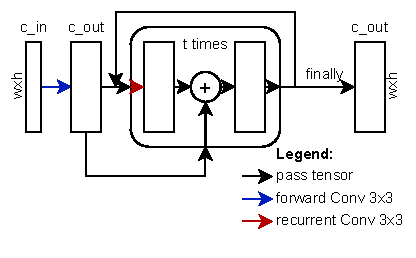
\includegraphics[width=\textwidth]{RCL}
		\caption{Recurrent Convolutional Layer (RCL)}
		\label{fig:rcl}
	\end{subfigure}
	\hfill
	\begin{subfigure}[b]{0.45\textwidth}
		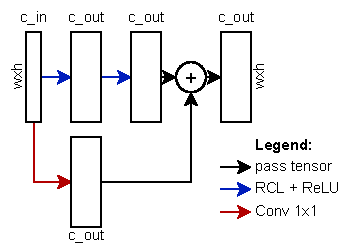
\includegraphics[width=\textwidth]{RRCU}
		\caption{Recurrent Residual Convolutional Unit (RRCU) (adopted from 
			\autocite[4]{R2UNet})}
		\label{fig:rrcu}
	\end{subfigure}
	\caption{Building blocks of R2U-Net}
	\label{fig:r2blocks}
\end{figure}

In the following we will elaborate on how the R2U-Net architecture as proposed 
in \autocite{R2UNet} has been implemented in this project. As the most basic 
building block of R2U-Net, a Recurrent Convolutional Layer
(RCL) as introduced in \autocite{RCNN} has been used. This is
illustrated in \autoref{fig:rcl}. Each rectangle in the following architecture 
figures represents a 3 dimensional tensor where its spatial (width $\times$ 
height) dimensions are denoted on its vertical line and its channel dimension 
is indicated on its horizontal line. An RCL generally consists of a 
feed-forward and a recurrent convolutional layer. To keep the spatial 
dimensions of the tensors intact, both of these convolutional layers used a 3x3 
kernel with a zero-padding of 1. As shown in \autoref{fig:rcl} the feed-forward 
layer maps the input tensor from the RCL's number of input channels $c_{in}$ to 
the 
RCL's number of output channels $c_{out}$. The recurrent layer subsequently 
retains $c_{out}$ for the channel dimension. Afterwards the feed-forward output 
tensor is added to the recurrent output tensor and this result is fed back into 
the recurrent layer. 
This procedure of applying the recurrent layer and adding the feed-forward 
output is repeated $t$ times until the tensor is finally output by the RCL. 
\autocite[4]{R2UNet}

The next building block of R2U-Net is the Recurrent Residual Convolutional Unit 
(RRCU) which is illustrated in \autoref{fig:rrcu}. It consists of two RCLs, 
each followed by a Rectified Linear Units (ReLU) activation function, where the 
first maps the channel dimension from the RRCU's $c_{in}$ to its $c_{out}$ and 
the second retains $c_{out}$. Finally, the residual connection adds the RRCU's 
input to the second RCL's output. However, as discussed in 
\autocite[3]{DeepResidual} the number of channels of the input have to be 
adapted through a linear transformation which is achieved by a convolutional 
layer with a 1x1 kernel. \autocite[4-5]{R2UNet}

\begin{figure}
	\centering
	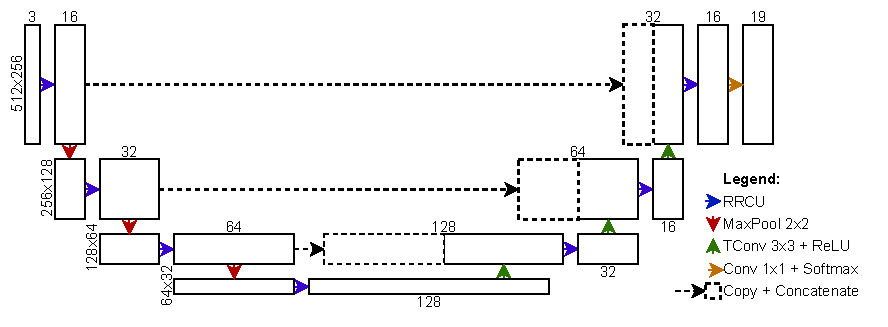
\includegraphics[width=\textwidth]{R2UNet}
	\caption{Baseline architecture of R2U-Net (adopted from 
	\autocite[3]{R2UNet})}
	\label{fig:r2unet}
\end{figure}

The total architecture of R2U-Net that uses these building blocks is shown in 
\autoref{fig:r2unet}. Starting from the input image on the left, the encoding 
path of the network alternatingly increases the number of channels using RRCUs 
and cuts the spatial dimensions in half with 2x2 Max Pooling layers. In the 
decoding path of the network the spatial dimensions of the tensors are doubled 
using transposed convolutional (TConv) layers followed by ReLU activation. 
These layers use 3x3 kernels, a padding of 1, a stride of 2 and an output 
padding of 1. The 
very first TConv layer also cuts the number of channels in half.
Moreover, the output tensors from the encoding path are copied and concatenated 
to the tensors from lower layers. These concatenated tensors are passed through 
RRCUs that quarter the number of channels except for the last layer where they 
are cut in half. To obtain the final segmentation map output, the network has a 
convolutional layer with 1x1 kernel and Softmax activation function.
\autocite[3-5]{R2UNet}

\subsubsection{BCDU-Net}

Besides R2U-Net the architecture BCDU-Net as proposed in \autocite{BCDUNet} has 
been investigated. The architecture and implementation details are described in 
the following.

\begin{figure}
	\centering
	\begin{subfigure}[b]{0.25\textwidth}
		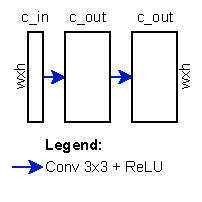
\includegraphics[width=\textwidth]{2ConvBlock}
		\caption{Double Convolutional Block (2Conv) (adopted from 
			\autocite[4]{BCDUNet})}
		\label{fig:2conv}
	\end{subfigure}
	\hfill
	\begin{subfigure}[b]{0.6\textwidth}
		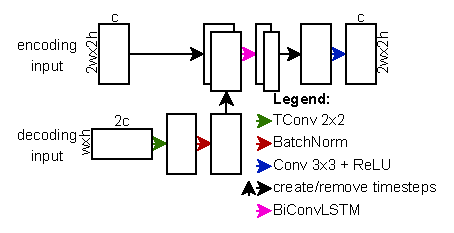
\includegraphics[width=\textwidth]{UpUnit}
		\caption{Upsampling Unit (UpUnit) of BCDU-Net (adopted from 
			\autocite[4]{BCDUNet})}
		\label{fig:upunit}
	\end{subfigure}
	\hfill
	\begin{subfigure}[b]{0.75\textwidth}
		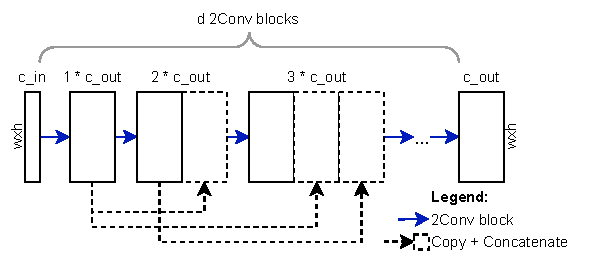
\includegraphics[width=\textwidth]{DenseConv}
		\caption{Dense Convolutional Layer (DenseConv) (adopted from 
			\autocite[4]{BCDUNet})}
		\label{fig:denseconv}
	\end{subfigure}
	\caption{Building blocks of BCDU-Net}
	\label{fig:bcdublocks}
\end{figure}

The most basic element of BCDU-Net is the Double Convolutional (2Conv) Block 
shown in \autoref{fig:2conv} which consists of two convolutional layers with a 
3x3 kernel and a zero-padding of 1, each with a ReLU activation. As before the 
first layer maps from the block's $c_{in}$ to its $c_{out}$ where the second 
one just retains $c_{out}$. \autocite[3]{BCDUNet}

Besides that the Dense Convolutional Layer (DenseConv) illustrated in 
\autoref{fig:denseconv} is constructed from these 2Conv blocks. The number of 
these blocks is given by the hyperparameter $d$. Each of these blocks outputs 
the layer's $c_{out}$ number of channels. While the first block takes the 
layer's $c_{in}$ number of channels as input, each $k$th subsequent block uses 
$k \cdot c_{out}$ number of channels as input. This emerges from the fact that 
the inputs are constructed by concatenating all previous output tensors. 
\autocite[3-4]{BCDUNet}

Additionally, BCDU-Net uses Bi-Directional Convolutional Long-short Term Memory 
(BiConvLSTM) cells as presented in \autocite[6-7]{BiConvLSTM}. These are built 
from convolutional LSTM cells which model both sequence information like 
classical LSTM cells \autocite{LSTM} and spatial information. This is done by 
replacing the matrix multiplications of LSTM by convolutional operations. In 
BiConvLSTM two of these convolutional LSTM cells are applied to the input in 
the forward and backward temporal direction respectively. The final output of 
BiConvLSTM is obtained by combining the hidden-state output tensors of both 
convolutional LSTM cells for each timestep. This is performed by passing the 
hidden states of both directions through each another convolutional layer and a 
hyperbolic tangent activation function.
\autocite[6-7]{BiConvLSTM}

Lastly, BCDU-Net has a special way of combining the tensors from the encoding 
and decoding path of the network. This is performed by the Upsampling Unit 
(UpUnit) shown in \autoref{fig:upunit}. Initially, it performs upsampling on 
the input from the decoding path using a TConv layer with 2x2 kernel and stride 
2. This layer doubles the spatial dimensions but cuts the number of channels in 
half so that its output has the same dimensionality as the input from the 
encoding path. The TConv layer is followed by a batch normalization layer. 
Subsequently its output is concatenated with the encoding input along a new 
tensor dimension representing timesteps. These are fed into a BiConvLSTM that 
cuts the number of channels in half. Finally, the timestep dimension of the 
tensors is collapsed back into the channel dimension and passed through a 3x3 
convolutional layer with a zero-padding of 1 and ReLU activation. 
\autocite[3-4]{BCDUNet}

\begin{figure}
	\centering
	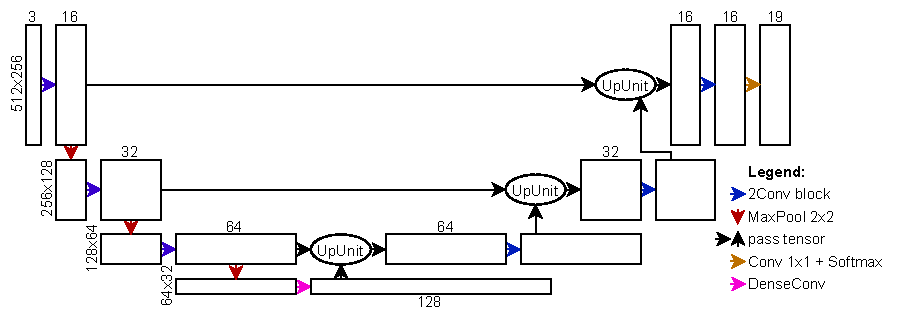
\includegraphics[width=\textwidth]{BCDUNet}
	\caption{Baseline architecture of BCDU-Net (adopted from 
		\autocite[4]{BCDUNet})}
	\label{fig:bcdunet}
\end{figure}

The overall architecture of BCDU-Net is shown in \autoref{fig:bcdunet}. In the 
encoding part it uses 2Conv blocks to increase the number of channels and 2x2 
Max Pooling to cut the spatial dimensions in half. However, the very last 
encoding step is performed with a DenseConv Layer. In the decoding part it uses 
the aforementioned UpUnit to combine tensors from the encoding and decoding 
part. Each UpUnit is followed by another 2Conv block that retains the number of 
channels. 
As in R2U-Net, the final layer is a convolutional layer with a 1x1 kernel and 
Softmax activation function to obtain the segmentation map. 
\autocite[3-4]{BCDUNet}

\subsection{Training configuration}
Both architectures were trained with an Adam optimizer \autocite{adam} with 
default betas and a 
learning rate that was tuned for convergence. Further, cross entropy was used 
as a loss function. Moreover, early stopping with a 
patience of 7 was used, so that the model training stopped when no improvement 
of the validation loss was achieved over the last 7 epochs. For both 
architectures the number of channels was varied and the batch size was 
adjusted accordingly to match GPU memory limitations. Additionally, the 
number of timesteps $t$ in R2U-Net and the depth of the DenseConv layer $d$ in 
BCDU-Net were tuned. Details are presented in \autoref{sec:results}.

\subsection{Evaluation metrics}
Similar to the evaluation in \autocite{R2UNet}, the final evaluation of both 
network architectures was performed using the binary classification metrics 
sensitivity (SE), specificity (SP), F1-score/Dice coefficient (DC) and Jaccard 
similarity (JS). On a per-pixel basis, these can be formulated in terms 
of the number of true positives (TP), false positives (FP), true negatives (TN) 
and false negatives (FN). According to \autocite[6]{R2UNet} 
\autocite{DiceJaccard} \autocite{SegMetrics} the metrics are defined as:

\begin{align}
	SE &= \frac{TP}{TP + FN}\\
	SP &= \frac{TN}{TN + FP}\\
	F1 = DC &= \frac{2TP}{2TP + FN + FP}\\
	JS &= \frac{TP}{TP + FN + FP}
\end{align}

Since these metrics only work for binary classification they were computed for 
each class in a one-vs-the-rest fashion. Total metrics were obtained by 
averaging 
over all individual class' metrics. Moreover, accuracy (AC) was directly 
computed as a total metric, representing the overall proportion of correctly 
classified pixels. Naturally, all of these metrics were computed on our test 
set containing 500 images.

\section{Results}
\label{sec:results}
\begin{table}
	\caption{Hyperparameter tuning experiments for R2U-Net}
	\label{tab:r2unet-tuning}
	\centering
	\begin{tabular}{
			|>{\raggedleft\arraybackslash}p{0.4cm}
			|>{\raggedright\arraybackslash}p{5.8cm}
			|>{\raggedleft\arraybackslash}p{0.3cm}
			|>{\raggedleft\arraybackslash}p{0.8cm}
			|>{\raggedleft\arraybackslash}p{1.2cm}
			|>{\raggedleft\arraybackslash}p{1.0cm}
			|>{\raggedleft\arraybackslash}p{1.4cm}
		|}
		\hline 
		\textbf{No.} & \textbf{Architecture (channels)} & \textbf{t} & 
		\textbf{Batch Size} & 
		\textbf{Learning Rate} & \textbf{Epochs} & \textbf{Validation Loss}\\ 
		\hline 
		\hline 
		% base-line
		1 & 3 $\rightarrow$ 16 $\rightarrow$ 32 $\rightarrow$ 64 $\rightarrow$ 
		128 $\rightarrow$ 64 $\rightarrow$ 32 $\rightarrow$ 16 $\rightarrow$ 19 
		& 2 & 32 & $10^{-3}$ & 60 & \textbf{0.3032} \\ 
		% more timesteps
		\hline 
		2 & 3 $\rightarrow$ 16 $\rightarrow$ 32 $\rightarrow$ 64 $\rightarrow$ 
		128 $\rightarrow$ 64 $\rightarrow$ 32 $\rightarrow$ 16 $\rightarrow$ 19 
		& 3 & 32 & $10^{-3}$ & 9 & 1.0523 \\ 
		\hline 
		3 & 3 $\rightarrow$ 16 $\rightarrow$ 32 $\rightarrow$ 64 $\rightarrow$ 
		128 $\rightarrow$ 64 $\rightarrow$ 32 $\rightarrow$ 16 $\rightarrow$ 19 
		& 3 & 32 & $10^{-4}$ & 162 & 0.4012 \\
		\hline 
		% more channels
		4 & 3 $\rightarrow$ 32 $\rightarrow$ 64 $\rightarrow$ 128 $\rightarrow$ 
		256 $\rightarrow$ 128 $\rightarrow$ 64 $\rightarrow$ 32 $\rightarrow$ 
		19 & 2 & 20 & $10^{-3}$ & 17 & 0.4678 \\
		\hline 
		5 & 3 $\rightarrow$ 32 $\rightarrow$ 64 $\rightarrow$ 128 $\rightarrow$ 
		256 $\rightarrow$ 128 $\rightarrow$ 64 $\rightarrow$ 32 $\rightarrow$ 
		19 & 2 & 20 & $10^{-4}$ & 66 & 0.3282 \\
		\hline 
	\end{tabular} 
\end{table}

\autoref{tab:r2unet-tuning} shows the conducted experiments to tune the 
hyperparameters of R2U-Net with their respective validation losses as a 
performance measure. Further, the number of training epochs before early 
stopping is shown as a metric for the training time needed. Interestingly, the 
baseline experiment 1 achieved the overall best performance while converging in 
a reasonable amount of time. In contrast to that experiment 2, where the number 
of timesteps was increased, did not converge properly and stopped very early 
with a high loss. This was fixed by a lower learning rate in experiment 3, 
however, this led to a very long training time and still a worse loss than 
experiment 1. Moreover, increasing the number of channels, as done in 
experiment 4 and 5, could not improve the performance either. Once again the 
learning rate was reduced in experiment 5 to achieve a lower loss but the 
training time remained reasonable this time.

\begin{table}
	\caption{Hyperparameter tuning experiments for BCDU-Net}
	\label{tab:bcdunet-tuning}
	\centering
	\begin{tabular}{
			|>{\raggedleft\arraybackslash}p{0.4cm}
			|>{\raggedright\arraybackslash}p{5.8cm}
			|>{\raggedleft\arraybackslash}p{0.3cm}
			|>{\raggedleft\arraybackslash}p{0.8cm}
			|>{\raggedleft\arraybackslash}p{1.2cm}
			|>{\raggedleft\arraybackslash}p{1.0cm}
			|>{\raggedleft\arraybackslash}p{1.4cm}
			|}
		\hline 
		\textbf{No.} & \textbf{Architecture (channels)} & \textbf{d} & 
		\textbf{Batch Size} & 
		\textbf{Learning Rate} & \textbf{Epochs} & \textbf{Validation Loss}\\  
		\hline 
		\hline 
		% shallow dense layer
		6 & 3 $\rightarrow$ 16 $\rightarrow$ 32 $\rightarrow$ 64 $\rightarrow$ 
		128 $\rightarrow$ 64 $\rightarrow$ 32 $\rightarrow$ 16 $\rightarrow$ 19 
		& 1 & 25 & $10^{-3}$ & 24 & 0.4194 \\  
		\hline 
		% base-line
		7 & 3 $\rightarrow$ 16 $\rightarrow$ 32 $\rightarrow$ 64 $\rightarrow$ 
		128 $\rightarrow$ 64 $\rightarrow$ 32 $\rightarrow$ 16 $\rightarrow$ 19 
		& 3 & 25 & $10^{-3}$ & 31 & \textbf{0.3792} \\  
		\hline 
		8 & 3 $\rightarrow$ 16 $\rightarrow$ 32 $\rightarrow$ 64 $\rightarrow$ 
		128 $\rightarrow$ 64 $\rightarrow$ 32 $\rightarrow$ 16 $\rightarrow$ 19 
		& 3 & 25 & $10^{-4}$ & 47 & 0.5085 \\ 
		\hline 
		% more channels
		9 & 3 $\rightarrow$ 32 $\rightarrow$ 64 $\rightarrow$ 128 
		$\rightarrow$ 256 $\rightarrow$ 128 $\rightarrow$ 64 $\rightarrow$ 32 
		$\rightarrow$ 19 
		& 3 & 12 & $10^{-3}$ & 17 & 0.5956 \\ 
		\hline 
		10 & 3 $\rightarrow$ 32 $\rightarrow$ 64 $\rightarrow$ 128 
		$\rightarrow$ 256 $\rightarrow$ 128 $\rightarrow$ 64 $\rightarrow$ 32 
		$\rightarrow$ 19 
		& 3 & 12 & $10^{-4}$ & 13 & 0.5311 \\ 
		\hline 
		11 & 3 $\rightarrow$ 32 $\rightarrow$ 64 $\rightarrow$ 128 
		$\rightarrow$ 
		256 $\rightarrow$ 128 $\rightarrow$ 64 $\rightarrow$ 32 $\rightarrow$ 
		19 
		& 3 & 12 & $2 \cdot 10^{-5}$ & 33 & 0.6202 \\ 
		\hline 
	\end{tabular} 
\end{table}

Similarly, \autoref{tab:bcdunet-tuning} shows the hyperparameter tuning 
experiments for BCDU-Net with their validation losses and epochs. It 
illustrates that for BCDU-Net convergence was achieved with rather few epochs 
and thus the training times always remained reasonable. This is possibly caused 
by the use of batch normalization layers which according to 
\autocite{batchNormHelps} speeds up training by smoothing the loss landscape. 
Additionally, the batch sizes had to be lower for BCDU-Net than for R2U-Net due 
to its higher memory requirements caused by its more advanced structure.
Moreover, we similarly to \autocite[5]{BCDUNet} observed that increasing the 
depth of the dense convolutional layer improves the performance as seen in 
experiment 6 and 7. Experiment 7 also shows the best performance for BCDU-Net. 
Neither further reducing of the learning rate (experiment 8) nor increasing the 
number of channels while tuning the learning rate (experiment 9 - 11) 
improved upon its validation loss. Especially for experiments 9 - 11 this could 
possibly be caused by the smaller batch size which potentially makes gradients 
too imprecise.

\begin{table}
	\caption{Total evaluation metrics for best R2U-Net and best BCDU-Net}
	\label{tab:r2-vs-bcd}
	\centering
	\begin{tabular}{
			|>{\raggedright\arraybackslash}p{3cm}
			|>{\raggedright\arraybackslash}p{1cm}
			|>{\raggedright\arraybackslash}p{1cm}
			|>{\raggedright\arraybackslash}p{1cm}
			|>{\raggedright\arraybackslash}p{1cm}
			|>{\raggedright\arraybackslash}p{1cm}
			|}
		\hline
		\textbf{Architecture} & \textbf{SE} & \textbf{SP} & \textbf{DC} & 
		\textbf{JS} 
		& \textbf{AC} \\ \hline
		\hline
		R2U-Net & 0.4625 & 0.9935 & 0.4817 & 0.3888 & 0.8956 \\ \hline
		BCDU-Net & 0.3721 & 0.9919 & 0.3779 & 0.3097 & 0.8705 \\ \hline
	\end{tabular} 
\end{table}

Comparing the validation losses of the best R2U-Net and BCDU-Net, we observe 
that R2U-Net performs better. This is also the case for the practical 
evaluation metrics shown in \autoref{tab:r2-vs-bcd}. This is contrary to the 
results obtained in \autocite{BCDUNet} for medical datasets and could possibly 
be caused by the different data domain, the higher number of classes or 
differences in the implementation details of the network. Furthermore, it is 
also possible that our experiments suffered from unlucky initialization or 
insufficient hyperparameter tuning. Nevertheless, both network architectures 
achieved reasonable accuracies. Moreover, SE, DC and JS are pretty low in 
\autoref{tab:r2-vs-bcd} when compared to \autocite{R2UNet} or 
\autocite{BCDUNet}. In contrast to that, SP is still very high. To get further 
insights into this behavior we will investigate the individual class' 
performance in the following.

\begin{table}
	\caption{Class-wise performance for best R2U-Net}
	\label{tab:r2-best}
	\centering
	\begin{tabular}{
			|>{\raggedright\arraybackslash}p{3cm}
			|>{\raggedright\arraybackslash}p{1cm}
			|>{\raggedright\arraybackslash}p{1cm}
			|>{\raggedright\arraybackslash}p{1cm}
			|>{\raggedright\arraybackslash}p{1cm}
			|}
		\hline
		\textbf{Class} & \textbf{SE} & \textbf{SP} & \textbf{DC} & 
		\textbf{JS} \\ \hline
		\hline
		road & 0.9776 & 0.983 & 0.9748 & 0.9508 \\ \hline
		sidewalk & 0.7887 & 0.9869 & 0.7817 & 0.6416 \\ \hline
		building & 0.9285 & 0.9605 & 0.8975 & 0.8141 \\ \hline
		wall & 0.2647 & 0.9972 & 0.3225 & 0.1922 \\ \hline
		fence & 0.1945 & 0.9963 & 0.2376 & 0.1348 \\ \hline
		pole & 0.3168 & 0.9983 & 0.4433 & 0.2848 \\ \hline
		traffic light & 0.0871 & 0.9998 & 0.1484 & 0.0801 \\ \hline
		traffic sign & 0.2127 & 0.9995 & 0.3298 & 0.1974 \\ \hline
		vegetation & 0.9296 & 0.9806 & 0.9194 & 0.8508 \\ \hline
		terrain & 0.5511 & 0.998 & 0.6149 & 0.444 \\ \hline
		sky & 0.9591 & 0.997 & 0.9378 & 0.8829 \\ \hline
		person & 0.6504 & 0.9938 & 0.6136 & 0.4426 \\ \hline
		rider & 0.0015 & 1.0 & 0.0029 & 0.0015 \\ \hline
		car & 0.9302 & 0.991 & 0.9037 & 0.8242 \\ \hline
		truck & 0.4287 & 0.9959 & 0.3062 & 0.1808 \\ \hline
		bus & 0.0313 & 0.9999 & 0.0597 & 0.0308 \\ \hline
		train & 0.0229 & 0.9997 & 0.0361 & 0.0184 \\ \hline
		motorcycle & 0.0465 & 0.9999 & 0.0791 & 0.0412 \\ \hline
		bicycle & 0.4657 & 0.9982 & 0.5439 & 0.3735 \\ \hline
	\end{tabular} 
\end{table}

\begin{table}
	\caption{Class-wise performance for best BCDU-Net}
	\label{tab:bcd-best}
	\centering
	\begin{tabular}{
			|>{\raggedright\arraybackslash}p{3cm}
			|>{\raggedright\arraybackslash}p{1cm}
			|>{\raggedright\arraybackslash}p{1cm}
			|>{\raggedright\arraybackslash}p{1cm}
			|>{\raggedright\arraybackslash}p{1cm}
			|}
		\hline
		\textbf{Class} & \textbf{SE} & \textbf{SP} & \textbf{DC} & 
		\textbf{JS} \\ \hline
		\hline
		road & 0.9669 & 0.9821 & 0.9685 & 0.939 \\ \hline
		sidewalk & 0.7632 & 0.9827 & 0.7387 & 0.5857 \\ \hline
		building & 0.916 & 0.9446 & 0.8669 & 0.7651 \\ \hline
		wall & 0.0336 & 0.9994 & 0.0607 & 0.0313 \\ \hline
		fence & 0.0235 & 0.9977 & 0.0361 & 0.0184 \\ \hline
		pole & 0.2105 & 0.9975 & 0.3061 & 0.1807 \\ \hline
		traffic light & 0.0164 & 0.9998 & 0.0299 & 0.0152 \\ \hline
		traffic sign & 0.1034 & 0.9997 & 0.1789 & 0.0982 \\ \hline
		vegetation & 0.8989 & 0.9818 & 0.9053 & 0.827 \\ \hline
		terrain & 0.4083 & 0.9982 & 0.5023 & 0.3354 \\ \hline
		sky & 0.9594 & 0.9957 & 0.9209 & 0.8535 \\ \hline
		person & 0.628 & 0.9868 & 0.4771 & 0.3133 \\ \hline
		rider & 0.0 & 1.0 & 0.0001 & 0.0 \\ \hline
		car & 0.9081 & 0.9814 & 0.8352 & 0.717 \\ \hline
		truck & 0.0187 & 0.9998 & 0.0344 & 0.0175 \\ \hline
		bus & 0.0001 & 1.0 & 0.0002 & 0.0001 \\ \hline
		train & 0.0048 & 0.9998 & 0.0081 & 0.0041 \\ \hline
		motorcycle & 0.0 & 1.0 & 0.0 & 0.0 \\ \hline
		bicycle & 0.2101 & 0.999 & 0.3099 & 0.1834 \\ \hline
	\end{tabular} 
\end{table}

The per-class binary metrics for R2U-Net and BCDU-Net are shown in 
\autoref{tab:r2-best} and \autoref{tab:bcd-best} respectively. If compared to 
\autocite[2]{Cordts2016Cityscapes}, they show that the performance on classes 
that cover large areas in the images is very good. Examples for such classes 
would be road, building, vegetation, car and sky. However, very infrequent 
classes are almost never predicted and thus have close to zero SE, DC and JS. 
For instace, this happens for the classes rider, motorcycle, bus and traffic 
light. This bad performance on the infrequent classes also explains the rather 
low average scores in \autoref{tab:r2-vs-bcd}. Regrading SP, the per-class 
results show almost perfect scores for all classes which also explains the very 
high average SP score for both models. However, in contrast to a true binary 
image segmentation problem the SP score is not very meaningful here due to the 
large number of classes and the 
one-vs-the-rest evaluation strategy. Since the negative class i.e. ``the rest'' 
consists of 18 classes each time, the network can misclassify a pixel as any of 
these 18 classes and still have a correct negative prediction leading to a high 
SP for the positive class under investigation.

Finally, we tried to tackle the problem of bad performance on infrequent 
classes. This behavior possibly is an artifact of the used loss function which 
does not account for different class frequencies. Therefore, we re-executed 
experiment 1 with a cross entropy loss that is weighted by the inverse class 
frequencies and once again tuned the learning rate. While this could 
significantly improve the performance on the rare classes it also notably 
decreased the performance on the frequent classes. On average this lead to 
slightly worse SE (0.465), DC (0.3026) and JS (0.2141) scores and a 
significantly worse accuracy (0.5878). Therefore, we concluded that solely a 
weighted loss does not fix the problem.

\section{Conclusion}
\label{sec:conclusion}
In summary, we observed that R2U-Net performed better than BCDU-Net in our 
experiments. Furthermore, increasing the number of channels did not improve the 
performance for both architectures. This is also true for R2U-Net's number of 
timesteps $t$. Only the increased depth $d$ of BCDU-Net's DenseConv layer had a 
positive effect on the performance. Additionally, both architectures struggled 
to classify objects correctly that only cover few pixels which significantly 
decreased the average performance over all classes. This could not really 
be fixed since training with a weighted loss function significantly degraded 
the performance for frequent classes.

For future work, the investigated architectures could be varied even more
in their configuration (e.g. number of channels) and trained with different 
initializations. More interestingly, they could also be architecturally varied 
in e.g. the placement of activation functions, normalization layers or by 
introducing entirely new units. Furthermore, different loss functions and 
further techniques should be investigated to improve the performance on 
infrequent classes.

\printbibliography

\end{document}
